\begin{frame}
  \frametitle{Werkwijze}

  \LaTeX~is \emph{geen programma}, het is een (programmeer)taal en document preparation system. Abstract gezien doen we het volgende:
  \begin{enumerate}
    \item we schrijven code;
    \item we geven deze aan een programma (\texttt{pdflatex} in ons geval) dat de code begrijpt;
    \item we krijgen output (een~\texttt{pdf} of errors).
  \end{enumerate}
\end{frame}

\begin{frame}
  \frametitle{Editor}

  Aan de tweede en derde stap kunnen we weinig veranderen, de eerste kunnen we w\'el zo aangenaam mogelijk proberen te maken door:
  \begin{itemize}
    \item zo weinig mogelijk zelf te moeten typen;
    \item syntax highlighting;
    \item errors markeren;
	  \item bad boxes aanduiden;
    \item templates voor veelgebruikte documenten;
    \item \ldots
  \end{itemize}
\end{frame}

\begin{frame}
  \frametitle{Thuis}

  Moet je \emph{eerst} zelf MiK\TeX~(of \TeX\ Live) installeren, download hiervoor de Basic MiK\TeX~2.9 installer van \href{http://miktex.org/2.9/setup}{miktex.org}. Linuxgebruikers: sowieso \TeX\ Live.

  Moet je \emph{vervolgens} je favoriete \LaTeX~editor installeren. Aangezien jullie nog geen voorkeuren hebben wordt dit~\TeX maker. Download de installatiebestanden op \url{http://xm1math.net/texmaker/} en na installatie zou alles moeten werken.
  \pause
  \begin{exampleblock}{Alternatieven}
    Ook te overwegen: \TeX studio, \TeX works (bijgeleverd met MiK\TeX), \TeX nicCenter (oud maar populair), \ldots
  \end{exampleblock}
\end{frame}

\begin{frame}
  \frametitle{In de computerklas}

  MiK\TeX~is ge\"installeerd dus daar moeten we ons geen zorgen over maken. Maar hoe \TeX maker gebruiken?

  Download hiervoor de \emph{stand-alone versie}, het bestand heet \texttt{texmakerwin32usb.zip} en pak dit uit. Open nu \texttt{texmaker.exe}

  \pause
  \begin{exampleblock}{Thuis}
    Enkel in de computerklas gebruiken we de stand-alone versie, thuis mag je het programma gerust installeren.
  \end{exampleblock}
\end{frame}

\begin{frame}
  \frametitle{Screenshot}
  
  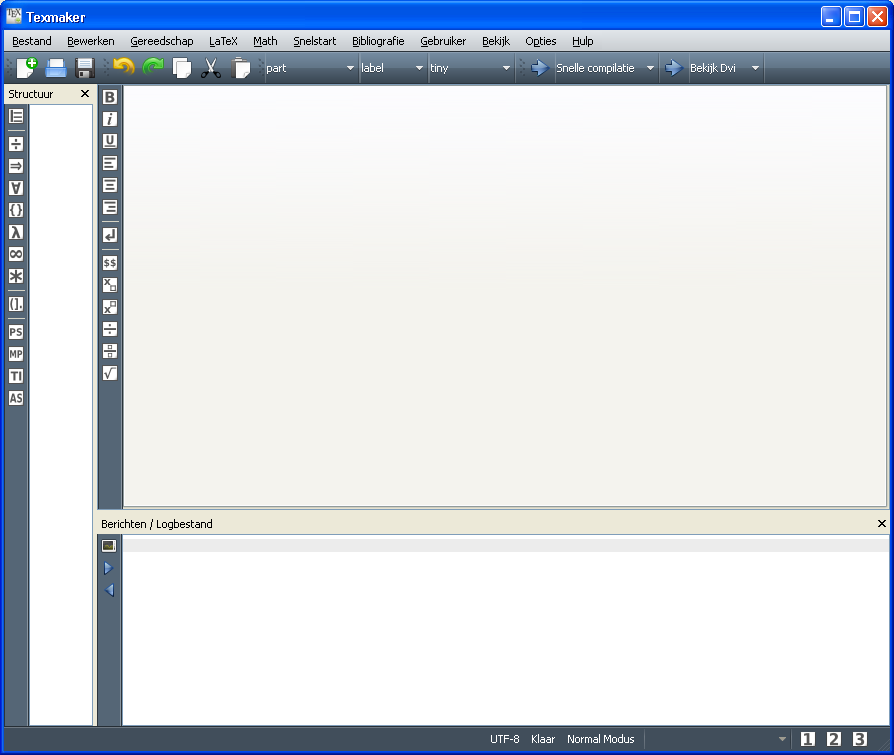
\includegraphics[scale=.2]{screenshot-1.png}
\end{frame}

\begin{frame}[fragile]
  \frametitle{Instellingen wijzigen}

  \begin{enumerate}
    \item ga naar Opties > Texmaker instellen
    \item plaats het volledige pad naar \texttt{pdflatex} bij PdfLaTeX
	  \begin{verbatim}
"C:/Program Files/MikTeX 2.9/miktex/bin/pdflatex.exe"
[...] -interaction=nonstopmode %.tex
	  \end{verbatim}
  \item plaats het volledige pad naar \texttt{bibtex} bij BibTex en verwijder \texttt{.aux}
	  \begin{verbatim}
"C:/Program Files/MikTeX 2.9/miktex/bin/bibtex.exe" %
	  \end{verbatim}
  \end{enumerate}
\end{frame}

\begin{frame}[fragile]
  \frametitle{Test}
  Typ volgende code over en druk op \texttt{F1}. Er zou iets moeten verschijnen.
  \inputminted{latex}{test-1.tex}
\end{frame}
